\textit{Results from the experiments that were considered relevant are presented here.}

\section{JNI}

% \begin{figure}
%     \begin{tikzpicture}
%         \begin{axis}[
%             xlabel={Block size},
%             ylabel={Time (ms)},
%             width=0.70\linewidth,
%             legend pos=south east,
%             scaled y ticks = false,
%         ]
%         \addplot [error bars/.cd, y dir=both, error bar style={red}, y explicit] coordinates {
%                 (16, 6.5035) +- (0.1, 0.1)
%                 (32, 5.2657) +- (0.1, 0.1)
%                 (64, 5.7065) +- (0.1, 0.1)
%                 (128, 6.1961) +- (0.1, 0.1)
%                 (256, 6.8872) +- (0.1, 0.1)
%                 (512, 9.7327) +- (0.1, 0.1)
%                 % (1024, 6.7378) +- (0.1, 0.1)
%                 % (2048, 5.8212) +- (0.1, 0.1)
%                 % (4096, 6.2328) +- (0.1, 0.1)
%                 % (8192, 5.6459) +- (0.1, 0.1)
%                 % (16384, 8.1388) +- (0.1, 0.1)
%                 % (32768, 10.2952) +- (0.1, 0.1)
%                 % (65536, 14.8090) +- (0.1, 0.1)
%         };
%         \addplot [error bars/.cd, y dir=both, error bar style={red}, y explicit] coordinates {
%                 (16, 2.4582) +- (0.1, 0.1)
%                 (32, 2.1875) +- (0.1, 0.1)
%                 (64, 2.1444) +- (0.1, 0.1)
%                 (128, 2.4097) +- (0.1, 0.1)
%                 (256, 2.2082) +- (0.1, 0.1)
%                 (512, 2.2379) +- (0.1, 0.1)
%                 % (1024, 2.2570) +- (0.1, 0.1)
%                 % (2048, 2.2917) +- (0.1, 0.1)
%                 % (4096, 2.2605) +- (0.1, 0.1)
%                 % (8192, 2.2291) +- (0.1, 0.1)
%                 % (16384, 2.2517) +- (0.1, 0.1)
%                 % (32768, 2.2500) +- (0.1, 0.1)
%                 % (65536, 2.1252) +- (0.1, 0.1)
%         };
%     \addplot [blue, error bars/.cd, y dir=both, error bar style={red}, y explicit] coordinates {
%                 (16, 2.8577) +- (0.1, 0.1)
%                 (32, 2.8438) +- (0.1, 0.1)
%                 (64, 2.8368) +- (0.1, 0.1)
%                 (128, 3.1840) +- (0.1, 0.1)
%                 (256, 3.0399) +- (0.1, 0.1)
%                 (512, 3.0243) +- (0.1, 0.1)
%                 % (1024, 4.0087) +- (0.1, 0.1)
%                 % (2048, 3.4426) +- (0.1, 0.1)
%                 % (4096, 3.4672) +- (0.1, 0.1)
%                 % (8192, 3.0208) +- (0.1, 0.1)
%                 % (16384, 5.0243) +- (0.1, 0.1)
%                 % (32768, 5.4063) +- (0.1, 0.1)
%                 % (65536, 6.4530) +- (0.1, 0.1)
%         };
%         % \legend{first-fit,best-fit,worst-fit,quick-fit,stdlib}
%         \end{axis}
%     \end{tikzpicture}
% \end{figure}

% \begin{figure}
%     \input{Data/results/JNI/Benchmark_vector.tex}
% \end{figure}

\begin{table}
    \centering
    \label{tab:jni:common}
    \caption{Results from the JNI tests, Time (ns)}
    \rowcolors{1}{}{lightgray}
\begin{tabular}{lcccc}\toprule
\textbf{Block size}  & \textbf{No params} & \textbf{Vector} & \textbf{Convert} & \textbf{Columbia}\\\midrule
\textbf{16}  & 1.7922 $\pm$ 0.1392 & 1.9333 $\pm$ 0.1223 & 2.6052 $\pm$ 0.1004 & 4.1058 $\pm$ 0.3042\\
\textbf{32}  & 1.6983 $\pm$ 0.0220 & 2.8130 $\pm$ 1.7924 & 2.6006 $\pm$ 0.0370 & 3.9109 $\pm$ 0.0535\\
\textbf{64}  & 1.6755 $\pm$ 0.0149 & 1.6344 $\pm$ 0.1809 & 2.6630 $\pm$ 0.0425 & 3.9296 $\pm$ 0.0566\\
\textbf{128}  & 1.9604 $\pm$ 0.4978 & 1.2349 $\pm$ 0.1262 & 1.9375 $\pm$ 0.0843 & 3.0823 $\pm$ 0.0892\\
\textbf{256}  & 1.7292 $\pm$ 0.0694 & 1.3276 $\pm$ 0.2589 & 1.8141 $\pm$ 0.0276 & 3.0958 $\pm$ 0.0441\\
\textbf{512}  & 1.6916 $\pm$ 0.0110 & 1.2567 $\pm$ 0.1227 & 2.2818 $\pm$ 0.7011 & 3.1656 $\pm$ 0.0457\\
\textbf{1024}  & 2.0228 $\pm$ 0.5684 & 1.3167 $\pm$ 0.1341 & 6.3756 $\pm$ 8.4676 & 3.2896 $\pm$ 0.1396\\
\textbf{2048}  & 1.7218 $\pm$ 0.0288 & 1.5416 $\pm$ 0.1405 & 1.9099 $\pm$ 0.0898 & 3.4844 $\pm$ 0.1113\\
\textbf{4096}  & 1.1411 $\pm$ 0.0404 & 1.4010 $\pm$ 0.0788 & 2.0062 $\pm$ 0.1562 & 3.8562 $\pm$ 0.3197\\
\textbf{8192}  & 1.1105 $\pm$ 0.0078 & 1.4818 $\pm$ 0.0759 & 2.3671 $\pm$ 0.1897 & 3.8474 $\pm$ 0.4784\\
\textbf{16384}  & 1.1183 $\pm$ 0.0280 & 1.7308 $\pm$ 0.1043 & 2.5833 $\pm$ 0.1737 & 4.9724 $\pm$ 0.8955\\
\textbf{32768}  & 1.1162 $\pm$ 0.0084 & 2.2099 $\pm$ 0.1880 & 3.2062 $\pm$ 0.2029 & 5.3719 $\pm$ 0.2875\\
\textbf{65536}  & 1.7463 $\pm$ 1.2217 & 4.7474 $\pm$ 3.1960 & 4.3198 $\pm$ 0.2926 & 6.8136 $\pm$ 0.2499\\
\textbf{131072}  & 1.1027 $\pm$ 0.0141 & 2.6375 $\pm$ 0.1531 & 5.7004 $\pm$ 0.2681 & 9.6912 $\pm$ 1.4337\\
\textbf{262144} & 1.1006 $\pm$ 0.0118 & 3.3172 $\pm$ 0.1164 & 7.4630 $\pm$ 0.2309 & 10.2781 $\pm$ 0.2278\\
\bottomrule
\end{tabular}

\end{table}

\begin{table}
    \centering
    \caption{Java tests, Time(ms)}
    \resizebox{\columnwidth}{!}{
        \rowcolors{1}{}{lightgray}
\begin{tabular}{lrrr}\toprule
\textbf{Block size}  & \textbf{Columbia Iterative} & \textbf{Princeton Iterative} & \textbf{Princeton Recursive}\\\midrule
\textbf{16}  & 0.03 $\pm$ 0.0010 & 0.12 $\pm$ 0.0053 & 0.13 $\pm$ 0.0108\\
\textbf{32}  & 0.08 $\pm$ 0.0033 & 0.13 $\pm$ 0.1198 & 0.06 $\pm$ 0.0035\\
\textbf{64}  & 0.02 $\pm$ 0.0125 & 0.09 $\pm$ 0.0468 & 0.13 $\pm$ 0.0043\\
\textbf{128}  & 0.01 $\pm$ 0.0002 & 0.14 $\pm$ 0.0020 & 0.49 $\pm$ 0.0486\\
\textbf{256}  & 0.02 $\pm$ 0.0008 & 0.56 $\pm$ 0.0947 & 0.69 $\pm$ 0.0325\\
\textbf{512}  & 0.06 $\pm$ 0.0010 & 0.87 $\pm$ 0.0615 & 1.75 $\pm$ 0.1245\\
\textbf{1024}  & 0.14 $\pm$ 0.0061 & 1.74 $\pm$ 0.0676 & 3.76 $\pm$ 0.2328\\
\textbf{2048}  & 0.43 $\pm$ 0.0159 & 4.40 $\pm$ 0.2064 & 8.69 $\pm$ 0.4575\\
\textbf{4096}  & 1.20 $\pm$ 0.0355 & 9.67 $\pm$ 0.4694 & 25.02 $\pm$ 0.8491\\
\textbf{8192}  & 2.87 $\pm$ 0.0637 & 22.96 $\pm$ 1.1025 & 52.08 $\pm$ 1.3973\\
\textbf{16384}  & 6.32 $\pm$ 0.2066 & 58.38 $\pm$ 1.9484 & 112.30 $\pm$ 1.6050\\
\textbf{32768}  & 12.26 $\pm$ 0.5700 & 150.72 $\pm$ 1.0864 & 239.07 $\pm$ 2.5276\\
\textbf{65536}  & 24.98 $\pm$ 0.9069 & 356.98 $\pm$ 1.5864 & 522.74 $\pm$ 6.1660\\
\textbf{131072}  & 85.94 $\pm$ 1.6097 & 815.86 $\pm$ 3.4304 & 1144.88 $\pm$ 17.8736\\
\textbf{262144} & 274.51 $\pm$ 5.1129 & 2108.07 $\pm$ 27.5366 & 2638.05 $\pm$ 40.5424\\
\bottomrule
\end{tabular}

    }
\end{table}

\begin{table}
    \centering
    \caption{CPP tests, Time(ms)}
    \resizebox{\columnwidth}{!}{
        \rowcolors{1}{}{lightgray}
\begin{tabular}{lrrrr}\toprule
\textbf{Block size}  & \textbf{Columbia Iterative} & \textbf{KISS} & \textbf{Princeton Iterative} & \textbf{Princeton Recursive}\\\midrule
\textbf{16}  & 0.0072 $\pm$ 0.0002 & 0.0056 $\pm$ 0.0002 & 0.0097 $\pm$ 0.0006 & 0.0202 $\pm$ 0.0008\\
\textbf{32}  & 0.0086 $\pm$ 0.0006 & 0.0069 $\pm$ 0.0002 & 0.0132 $\pm$ 0.0002 & 0.0368 $\pm$ 0.0008\\
\textbf{64}  & 0.0083 $\pm$ 0.0008 & 0.0079 $\pm$ 0.0002 & 0.0214 $\pm$ 0.0008 & 0.0705 $\pm$ 0.0022\\
\textbf{128}  & 0.0115 $\pm$ 0.0006 & 0.0131 $\pm$ 0.0006 & 0.0342 $\pm$ 0.0008 & 0.1434 $\pm$ 0.0012\\
\textbf{256}  & 0.0200 $\pm$ 0.0008 & 0.0182 $\pm$ 0.0008 & 0.0627 $\pm$ 0.0008 & 0.2978 $\pm$ 0.0025\\
\textbf{512}  & 0.0366 $\pm$ 0.0006 & 0.0461 $\pm$ 0.0022 & 0.1225 $\pm$ 0.0006 & 0.6379 $\pm$ 0.0035\\
\textbf{1024}  & 0.0773 $\pm$ 0.0020 & 0.0992 $\pm$ 0.0172 & 0.2744 $\pm$ 0.0098 & 1.3437 $\pm$ 0.0086\\
\textbf{2048}  & 0.2604 $\pm$ 0.0123 & 0.2047 $\pm$ 0.0149 & 0.5257 $\pm$ 0.0035 & 2.8773 $\pm$ 0.0253\\
\textbf{4096}  & 0.7974 $\pm$ 0.0216 & 0.4022 $\pm$ 0.0123 & 1.1701 $\pm$ 0.0118 & 6.1206 $\pm$ 0.0598\\
\textbf{8192}  & 1.9326 $\pm$ 0.0519 & 1.2470 $\pm$ 0.0451 & 2.5845 $\pm$ 0.0410 & 13.2345 $\pm$ 0.1433\\
\textbf{16384}  & 4.2789 $\pm$ 0.1254 & 2.3713 $\pm$ 0.0962 & 5.4518 $\pm$ 0.1149 & 27.6080 $\pm$ 0.1784\\
\textbf{32768}  & 9.9388 $\pm$ 0.3203 & 6.7420 $\pm$ 0.2534 & 12.2266 $\pm$ 0.4831 & 55.1227 $\pm$ 1.2277\\
\textbf{65536}  & 23.1031 $\pm$ 0.7648 & 16.0281 $\pm$ 0.3542 & 27.2805 $\pm$ 0.9530 & 102.1585 $\pm$ 3.5262\\
\textbf{131072}  & 75.4942 $\pm$ 1.6429 & 41.7620 $\pm$ 0.5968 & 78.9501 $\pm$ 1.9300 & 231.2663 $\pm$ 6.7357\\
\textbf{262144} & 243.8496 $\pm$ 1.0072 & 102.1196 $\pm$ 1.0817 & 250.4870 $\pm$ 5.2771 & 494.7038 $\pm$ 13.6690\\
\bottomrule
\end{tabular}

    }
\end{table}

\begin{table}
    \centering
    \caption{CPP tests, Time(ms)}
    \resizebox{\columnwidth}{!}{
        \rowcolors{1}{}{lightgray}
\begin{tabular}{lrrrr}\toprule
\textbf{Block size}  & \textbf{Columbia Iterative} & \textbf{KISS} & \textbf{Princeton Iterative} & \textbf{Princeton Recursive}\\\midrule
\textbf{16}  & 0.0072 $\pm$ 0.0002 & 0.0056 $\pm$ 0.0002 & 0.0097 $\pm$ 0.0006 & 0.0202 $\pm$ 0.0008\\
\textbf{32}  & 0.0086 $\pm$ 0.0006 & 0.0069 $\pm$ 0.0002 & 0.0132 $\pm$ 0.0002 & 0.0368 $\pm$ 0.0008\\
\textbf{64}  & 0.0083 $\pm$ 0.0008 & 0.0079 $\pm$ 0.0002 & 0.0214 $\pm$ 0.0008 & 0.0705 $\pm$ 0.0022\\
\textbf{128} & 0.0115 $\pm$ 0.0006 & 0.0131 $\pm$ 0.0006 & 0.0342 $\pm$ 0.0008 & 0.1434 $\pm$ 0.0012\\
\bottomrule
\end{tabular}

    }
\end{table}

\begin{table}
    \centering
    \caption{NEON tests, Time(ms)}
    \rowcolors{1}{}{lightgray}
\begin{tabular}{lrr}\toprule
\textbf{Block size}  & \textbf{Iterative} & \textbf{Recursive}\\\midrule
\textbf{16}  & 0.005 $\pm$ 0.0004 & 0.010 $\pm$ 0.0006\\
\textbf{32}  & 0.005 $\pm$ 0.0002 & 0.015 $\pm$ 0.0010\\
\textbf{64}  & 0.005 $\pm$ 0.0002 & 0.018 $\pm$ 0.0014\\
\textbf{128}  & 0.008 $\pm$ 0.0002 & 0.028 $\pm$ 0.0016\\
\textbf{256}  & 0.013 $\pm$ 0.0008 & 0.054 $\pm$ 0.0076\\
\textbf{512}  & 0.034 $\pm$ 0.0006 & 0.096 $\pm$ 0.0014\\
\textbf{1024}  & 0.060 $\pm$ 0.0020 & 0.186 $\pm$ 0.0029\\
\textbf{2048}  & 0.192 $\pm$ 0.0176 & 0.365 $\pm$ 0.0082\\
\textbf{4096}  & 0.365 $\pm$ 0.0161 & 0.808 $\pm$ 0.0200\\
\textbf{8192}  & 1.005 $\pm$ 0.0129 & 1.613 $\pm$ 0.0278\\
\textbf{16384}  & 2.155 $\pm$ 0.0502 & 3.569 $\pm$ 0.0857\\
\textbf{32768}  & 4.789 $\pm$ 0.1543 & 7.600 $\pm$ 0.1878\\
\textbf{65536}  & 9.880 $\pm$ 0.2452 & 16.112 $\pm$ 0.3712\\
\textbf{131072}  & 27.815 $\pm$ 0.7146 & 34.165 $\pm$ 0.4722\\
\textbf{262144} & 63.185 $\pm$ 1.2662 & 74.074 $\pm$ 1.0666\\
\bottomrule
\end{tabular}

\end{table}

\begin{figure}
    \centering
    \caption{NEON line graph EXTRA}
    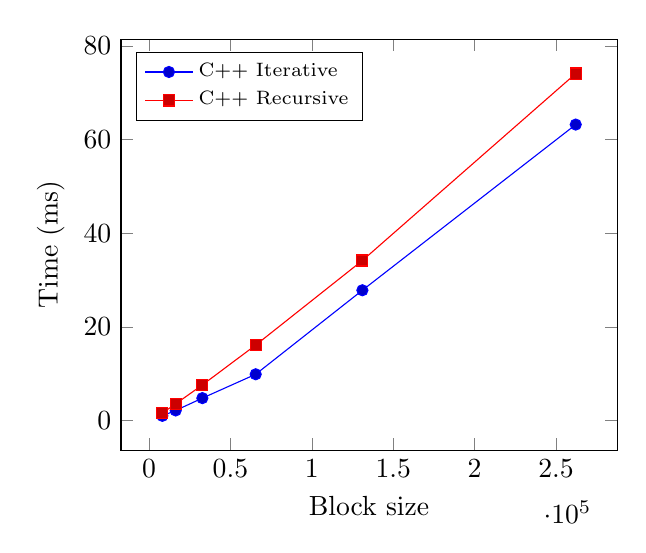
\begin{tikzpicture}
\begin{axis}[xlabel={Block size},ylabel={Time (ms)},width=0.65\linewidth,legend pos=north west,scaled y ticks = false,legend cell align=left,legend style={font=\scriptsize}]
\addplot coordinates {
(8192, 1.0051)
(16384, 2.1559)
(32768, 4.7898)
(65536, 9.8807)
(131072, 27.8158)
(262144, 63.1858)
};
\addplot coordinates {
(8192, 1.6133)
(16384, 3.5690)
(32768, 7.6009)
(65536, 16.1129)
(131072, 34.1650)
(262144, 74.0746)
};
\legend{C++ Iterative,C++ Recursive}
\end{axis}
\end{tikzpicture}

\end{figure}

\begin{figure}
    \centering
    \caption{Line graph EXTRA}
    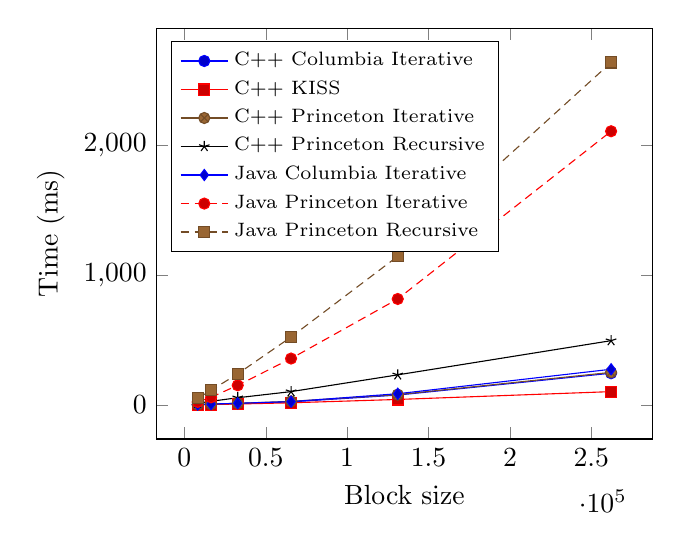
\begin{tikzpicture}
\begin{axis}[xlabel={Block size},ylabel={Time (ms)},width=0.65\linewidth,legend pos=north west,scaled y ticks = false,legend cell align=left,legend style={font=\scriptsize}]
\addplot coordinates {
(8192, 1.9326)
(16384, 4.2789)
(32768, 9.9388)
(65536, 23.1031)
(131072, 75.4942)
(262144, 243.8496)
};
\addplot coordinates {
(8192, 1.2470)
(16384, 2.3713)
(32768, 6.7420)
(65536, 16.0281)
(131072, 41.7620)
(262144, 102.1196)
};
\addplot coordinates {
(8192, 2.5845)
(16384, 5.4518)
(32768, 12.2266)
(65536, 27.2805)
(131072, 78.9501)
(262144, 250.4870)
};
\addplot coordinates {
(8192, 13.2345)
(16384, 27.6080)
(32768, 55.1227)
(65536, 102.1585)
(131072, 231.2663)
(262144, 494.7038)
};
\addplot coordinates {
(8192, 2.8726)
(16384, 6.3214)
(32768, 12.2634)
(65536, 24.9874)
(131072, 85.9483)
(262144, 274.5134)
};
\addplot coordinates {
(8192, 22.9609)
(16384, 58.3825)
(32768, 150.7299)
(65536, 356.9871)
(131072, 815.8607)
(262144, 2108.0771)
};
\addplot coordinates {
(8192, 52.0853)
(16384, 112.3024)
(32768, 239.0777)
(65536, 522.7409)
(131072, 1144.8802)
(262144, 2638.0547)
};
\legend{C++ Columbia Iterative,C++ KISS,C++ Princeton Iterative,C++ Princeton Recursive,Java Columbia Iterative,Java Princeton Iterative,Java Princeton Recursive}
\end{axis}
\end{tikzpicture}

\end{figure}

\begin{figure}
    \centering
    \caption{Line graph LARGE}
    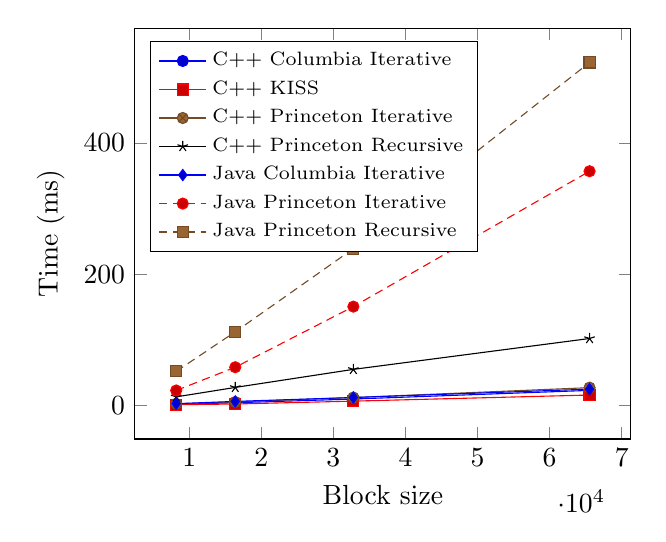
\begin{tikzpicture}
\begin{axis}[xlabel={Block size},ylabel={Time (ms)},width=0.65\linewidth,legend pos=north west,scaled y ticks = false,legend cell align=left,legend style={font=\scriptsize}]
\addplot coordinates {
(8192, 1.9326)
(16384, 4.2789)
(32768, 9.9388)
(65536, 23.1031)
};
\addplot coordinates {
(8192, 1.2470)
(16384, 2.3713)
(32768, 6.7420)
(65536, 16.0281)
};
\addplot coordinates {
(8192, 2.5845)
(16384, 5.4518)
(32768, 12.2266)
(65536, 27.2805)
};
\addplot coordinates {
(8192, 13.2345)
(16384, 27.6080)
(32768, 55.1227)
(65536, 102.1585)
};
\addplot coordinates {
(8192, 2.8726)
(16384, 6.3214)
(32768, 12.2634)
(65536, 24.9874)
};
\addplot coordinates {
(8192, 22.9609)
(16384, 58.3825)
(32768, 150.7299)
(65536, 356.9871)
};
\addplot coordinates {
(8192, 52.0853)
(16384, 112.3024)
(32768, 239.0777)
(65536, 522.7409)
};
\legend{C++ Columbia Iterative,C++ KISS,C++ Princeton Iterative,C++ Princeton Recursive,Java Columbia Iterative,Java Princeton Iterative,Java Princeton Recursive}
\end{axis}
\end{tikzpicture}

\end{figure}

\begin{figure}
    \centering
    \caption{CPP Line graph LARGE}
    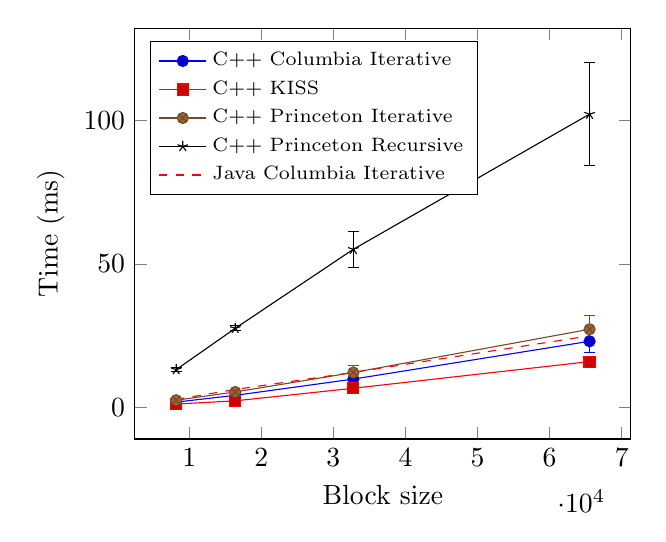
\begin{tikzpicture}
\begin{axis}[xlabel={Block size},ylabel={Time (ms)},width=0.65\linewidth,legend pos=north west,scaled y ticks = false,legend cell align=left,legend style={font=\scriptsize}]
\addplot+[error bars/.cd, y dir=both,y explicit] coordinates {
(8192, 1.9326) +- (0.2654, 0.2654)
(16384, 4.2789) +- (0.6399, 0.6399)
(32768, 9.9388) +- (1.6341, 1.6341)
(65536, 23.1031) +- (3.9019, 3.9019)
};
\addplot+[error bars/.cd, y dir=both,y explicit] coordinates {
(8192, 1.2470) +- (0.2301, 0.2301)
(16384, 2.3713) +- (0.4915, 0.4915)
(32768, 6.7420) +- (1.2931, 1.2931)
(65536, 16.0281) +- (1.8073, 1.8073)
};
\addplot+[error bars/.cd, y dir=both,y explicit] coordinates {
(8192, 2.5845) +- (0.2085, 0.2085)
(16384, 5.4518) +- (0.5858, 0.5858)
(32768, 12.2266) +- (2.4651, 2.4651)
(65536, 27.2805) +- (4.8616, 4.8616)
};
\addplot+[error bars/.cd, y dir=both,y explicit] coordinates {
(8192, 13.2345) +- (0.7311, 0.7311)
(16384, 27.6080) +- (0.9098, 0.9098)
(32768, 55.1227) +- (6.2636, 6.2636)
(65536, 102.1585) +- (17.9911, 17.9911)
};
\addplot+[style=dashed,color=red,mark=none] coordinates {
(8192, 2.8726) +- (0.3247, 0.3247)
(16384, 6.3214) +- (1.0542, 1.0542)
(32768, 12.2634) +- (2.9076, 2.9076)
(65536, 24.9874) +- (4.6266, 4.6266)
};
\legend{C++ Columbia Iterative , C++ KISS , C++ Princeton Iterative , C++ Princeton Recursive, Java Columbia Iterative}
\end{axis}
\end{tikzpicture}

\end{figure}

\section{FFT Libraries}

% \begin{figure}
%     \centering
%     \resizebox{\columnwidth}{!}{
%         \input{Data/results/FFT/barchart_65536.tex}
%     }
%     \label{tab:barchart:65536}
%     \caption{Bar chart for tests with block size 65536}
% \end{figure}
% Which is slowest and why (discussion)??

% Which is fastest and why (discussion)??

% Which tests triggered the GC??

\section{Optimizations}


